%%%%%%%%%%%%%%%%%%%%%%%%%%%%%%%%%%%%%%%%%%%%%%%%%%%%%%%%%%%%%%%%%%%%%%%%%%%%%%%%%%%%%%%%%%%%%%%%%%%%%%%%%%%%%%%%%%%%%%%%%%%%%%%%%%%%%%%%%%%%%%%%%%%%%%%%%%%
% This is just an example/guide for you to refer to when submitting manuscripts to Frontiers, it is not mandatory to use Frontiers .cls files nor frontiers.tex  %
% This will only generate the Manuscript, the final article will be typeset by Frontiers after acceptance.
%                                              %
%                                                                                                                                                         %
% When submitting your files, remember to upload this *tex file, the pdf generated with it, the *bib file (if bibliography is not within the *tex) and all the figures.
%%%%%%%%%%%%%%%%%%%%%%%%%%%%%%%%%%%%%%%%%%%%%%%%%%%%%%%%%%%%%%%%%%%%%%%%%%%%%%%%%%%%%%%%%%%%%%%%%%%%%%%%%%%%%%%%%%%%%%%%%%%%%%%%%%%%%%%%%%%%%%%%%%%%%%%%%%%

%%% Version 3.4 Generated 2018/06/15 %%%
%%% You will need to have the following packages installed: datetime, fmtcount, etoolbox, fcprefix, which are normally inlcuded in WinEdt. %%%
%%% In http://www.ctan.org/ you can find the packages and how to install them, if necessary. %%%

\documentclass[utf8]{frontiersSCNS}

%\setcitestyle{square} % for Physics and Applied Mathematics and Statistics articles
\usepackage{url,hyperref,lineno,microtype,subcaption}
\usepackage[onehalfspacing]{setspace}

\linenumbers


% BELOW TAKEN FROM rticles plos template
%
% amsmath package, useful for mathematical formulas
\usepackage{amsmath}
% amssymb package, useful for mathematical symbols
\usepackage{amssymb}

% hyperref package, useful for hyperlinks
\usepackage{hyperref}

% graphicx package, useful for including eps and pdf graphics
% include graphics with the command \includegraphics
\usepackage{graphicx}

% Sweave(-like)
\usepackage{fancyvrb}
\DefineVerbatimEnvironment{Sinput}{Verbatim}{fontshape=sl}
\DefineVerbatimEnvironment{Soutput}{Verbatim}{}
\DefineVerbatimEnvironment{Scode}{Verbatim}{fontshape=sl}
\newenvironment{Schunk}{}{}
\DefineVerbatimEnvironment{Code}{Verbatim}{}
\DefineVerbatimEnvironment{CodeInput}{Verbatim}{fontshape=sl}
\DefineVerbatimEnvironment{CodeOutput}{Verbatim}{}
\newenvironment{CodeChunk}{}{}

% cite package, to clean up citations in the main text. Do not remove.
\usepackage{cite}

\usepackage{color}

\providecommand{\tightlist}{%
  \setlength{\itemsep}{0pt}\setlength{\parskip}{0pt}}

% Below is from frontiers
%
\bibliographystyle{frontiersinSCNS}
% Use doublespacing - comment out for single spacing
%\usepackage{setspace}
%\doublespacing


% Leave a blank line between paragraphs instead of using \\


\def\keyFont{\fontsize{8}{11}\helveticabold }


%% ** EDIT HERE **
%% PLEASE INCLUDE ALL MACROS BELOW

%% END MACROS SECTION

% Pandoc citation processing
\newlength{\csllabelwidth}
\setlength{\csllabelwidth}{3em}
\newlength{\cslhangindent}
\setlength{\cslhangindent}{1.5em}
% for Pandoc 2.8 to 2.10.1
\newenvironment{cslreferences}%
  {}%
  {\par}
% For Pandoc 2.11+
\newenvironment{CSLReferences}[2] % #1 hanging-ident, #2 entry spacing
 {% don't indent paragraphs
  \setlength{\parindent}{0pt}
  % turn on hanging indent if param 1 is 1
  \ifodd #1 \everypar{\setlength{\hangindent}{\cslhangindent}}\ignorespaces\fi
  % set entry spacing
  \ifnum #2 > 0
  \setlength{\parskip}{#2\baselineskip}
  \fi
 }%
 {}
\usepackage{calc} % for calculating minipage widths
\newcommand{\CSLBlock}[1]{#1\hfill\break}
\newcommand{\CSLLeftMargin}[1]{\parbox[t]{\csllabelwidth}{#1}}
\newcommand{\CSLRightInline}[1]{\parbox[t]{\linewidth - \csllabelwidth}{#1}\break}
\newcommand{\CSLIndent}[1]{\hspace{\cslhangindent}#1}


\def\Authors{
  Maxwel C Oliveira\,\textsuperscript{1},
  Amit J Jhala\,\textsuperscript{2},
  Mark Bernards\,\textsuperscript{3},
  Chris Proctor\,\textsuperscript{2},
  Strahinja Stepanovic\,\textsuperscript{2},
  Rodrigo Werle\,\textsuperscript{1*}}

\def\Address{

  \textsuperscript{1} Department of Agronomy, University of
Wisconsin-Madison,  Madison,  Wisconsin,  United States
  
  \textsuperscript{2} Department of Agronomy and
Horticulture, University of
Nebraska-Lincoln,  Lincoln,  Nebraska,  United States
  
  \textsuperscript{3} Department of Agronomy, Western Illinois
University,  Macomb,  Illnois,  United States
  }

  
  \def\firstAuthorLast{Oliveira {et~al.}}
  
  
  
  
  
  
  
  
  \def\corrAuthor{Rodrigo Werle}\def\corrAddress{Department of Agronomy,
University of Wisconsin-Madison, United States\\1575 Linden
Dr\\Madison, Wisconsin, 53705 United
States}\def\corrEmail{\href{mailto:rwerle@uwisc.edu}{\nolinkurl{rwerle@uwisc.edu}}}
  


\begin{document}
\onecolumn
\firstpage{1}

\title[Short Title]{Adaptation of Palmer amaranth to croppins systems}
\author[\firstAuthorLast]{\Authors}
\address{} %This field will be automatically populated
\correspondance{} %This field will be automatically populated

\extraAuth{}% If there are more than 1 corresponding author, comment this line and uncomment the next one.
%\extraAuth{corresponding Author2 \\ Laboratory X2, Institute X2, Department X2, Organization X2, Street X2, City X2 , State XX2 (only USA, Canada and Australia), Zip Code2, X2 Country X2, email2@uni2.edu}


\maketitle

\begin{abstract}

Abstract length and content varies depending on article type. Refer to 
\url{http://www.frontiersin.org/about/AuthorGuidelines} for abstract requirement
and length according to article type.

%All article types: you may provide up to 8 keywords; at least 5 are mandatory.
\tiny
 \keyFont{ \section{Keywords:} Text Text Text Text Text Text Evolution Weed } 

\end{abstract}

\hypertarget{introduction}{%
\section*{Introduction}\label{introduction}}
\addcontentsline{toc}{section}{Introduction}

Palmer amaranth (\emph{Amaranthus palmeri}) is an indigenous species
from southwestern United States and northern Mexico. Palmer amaranth is
a C4 annual broadleaf forb within the \textbf{Amarantacea} family.
Palmer amaranth is currently considered one of the most troublesome weed
species in the United States.

\hypertarget{material-and-methods}{%
\section*{Material and Methods}\label{material-and-methods}}
\addcontentsline{toc}{section}{Material and Methods}

\hypertarget{plant-material-and-growing-conditions}{%
\subsection*{Plant material and growing
conditions}\label{plant-material-and-growing-conditions}}
\addcontentsline{toc}{subsection}{Plant material and growing conditions}

The study was performed with a \emph{A. palmeri} accession (Per1) from
Perkins County, Nebraska. Per1 accession collection is documented in
(Oliveira et al., 2021), with no reported herbicide resistance. Three
weeks prior to the field experiment, seeds were planted in plastic trays
containing potting-mix. Emerged seedlings (1 cm) were transplanted into
200 cm-3 plastic pots (a plant pot-1). Palmer amaranth seedlings were
supplied with adequate water and kept under greenhouse conditions at
Arlington, Clay Center, Lincoln, and Macomb; and kept outdoors in Grant.
Palmer amaranth seedlings were kept under greenhouse/outdoors until the
onset of the experiment (7 to 10 cm height).

\hypertarget{field-study}{%
\subsection*{Field study}\label{field-study}}
\addcontentsline{toc}{subsection}{Field study}

The experiment was conducted in 2018 and 2019 under field conditions at
five locations: Arlington (Washington County, Wisconsin), Clay Center
(Clay County, Nebraska), Grant (Perkins County, Nebraska), Lincoln
(Lancaster County, Nebraska), and Macomb (McDonough County, Illinois).

The experimental unit were adjacent 9.1 m wide (12 rows at 72.2 cm row
spacing) by 10.7 m long. Each experimental unit was planted with corn or
soybean, or left fallow. Palmer amaranth seedlings were transplanted to
the field experiment by making a whole in the soil (6 cm deep and 8 cm
wide); and gently transferring in the ground (potting mix + two
seedlings). After a week, if both plants were alive, one was eliminated.
There were two transplant timing: early (June 1\textsuperscript{st}) and
late (July 1\textsuperscript{st}). There were 24 Palmer amaranth plants
in each crop/fallow and timing, with a total of 144 plants. The study
was repeated twice.

After transplanting, Palmer amaranth flowering was monitored until the
end of the study. When a plant started flowering, the day was recorded,
plant sex was identified as male or female, and plant height was
measured from soil surface to the plant top. Then, aboveground plant
biomass was harvest near soil surface and oven dried at 65 C until
reaching constant weight before the weight of biomass (g
plant\textsuperscript{-1}) was recorded.

\hypertarget{statistical-analyses}{%
\subsection*{Statistical analyses}\label{statistical-analyses}}
\addcontentsline{toc}{subsection}{Statistical analyses}

The statistical analyses were performed using R statistical software
version 4.0.1.

The cumulative Palmer amaranth flowering estimation was determined using
a asymmetrical three parameter log logistic Weibull model of the drc
package (Ritz et al., 2015).

\[Y(x) = 0 + (d-0) exp (-exp(b(log(x)-e)))\] In this model, \emph{Y} is
the Palmer amaranth cumulative flowering, \emph{d} is the upper limit
(set to 100), and \emph{e} is the XXX, and \emph{x} day of year (doy).

The doy for 10, 50, and 90\% Palmer amaranth cumulative flowering were
determined using the \emph{ED} function of drc package. Also, the 10,
50, and 90\% Palmer amaranth cumulative flowering were compared among
crop/fallow and timings using the \emph{EDcomp} function of drc package.
The EDcomp function compares the ratio of cumulative flowering using
t-statistics, where P-value \textless{} 0.05 indicates that we fail to
reject the null hypothesis.

\hypertarget{results}{%
\section*{Results}\label{results}}
\addcontentsline{toc}{section}{Results}

\hypertarget{subsection-1}{%
\subsection*{Subsection 1}\label{subsection-1}}
\addcontentsline{toc}{subsection}{Subsection 1}

You can use \texttt{R} chunks directly to plot graphs.

\hypertarget{subsection-2}{%
\subsection*{Subsection 2}\label{subsection-2}}
\addcontentsline{toc}{subsection}{Subsection 2}

Frontiers requires figures to be submitted individually, in the same
order as they are referred to in the manuscript. Figures will then be
automatically embedded at the bottom of the submitted manuscript. Kindly
ensure that each table and figure is mentioned in the text and in
numerical order. Permission must be obtained for use of copyrighted
material from other sources (including the web). Please note that it is
compulsory to follow figure instructions. Figures which are not
according to the guidelines will cause substantial delay during the
production process.

\hypertarget{discussion}{%
\section{Discussion}\label{discussion}}

\hypertarget{disclosureconflict-of-interest-statement}{%
\section*{Disclosure/Conflict-of-Interest
Statement}\label{disclosureconflict-of-interest-statement}}
\addcontentsline{toc}{section}{Disclosure/Conflict-of-Interest
Statement}

The authors declare that the research was conducted in the absence of
any commercial or financial relationships that could be construed as a
potential conflict of interest.

\hypertarget{author-contributions}{%
\section*{Author Contributions}\label{author-contributions}}
\addcontentsline{toc}{section}{Author Contributions}

The statement about the authors and contributors can be up to several
sentences long, describing the tasks of individual authors referred to
by their initials and should be included at the end of the manuscript
before the References section.

\hypertarget{acknowledgments}{%
\section*{Acknowledgments}\label{acknowledgments}}
\addcontentsline{toc}{section}{Acknowledgments}

Funding:

\hypertarget{supplemental-data}{%
\section{Supplemental Data}\label{supplemental-data}}

Supplementary Material should be uploaded separately on submission, if
there are Supplementary Figures, please include the caption in the same
file as the figure. LaTeX Supplementary Material templates can be found
in the Frontiers LaTeX folder

\hypertarget{references}{%
\section{References}\label{references}}

A reference list should be automatically created here. However it won't.
Pandoc will place the list of references at the end of the document
instead. There are no convenient solution for now to force Pandoc to do
otherwise. The easiest way to get around this problem is to edit the
LaTeX file created by Pandoc before compiling it again using the
traditional LaTeX commands.

\hypertarget{figures}{%
\section*{Figures}\label{figures}}
\addcontentsline{toc}{section}{Figures}

\begin{figure}

{\centering 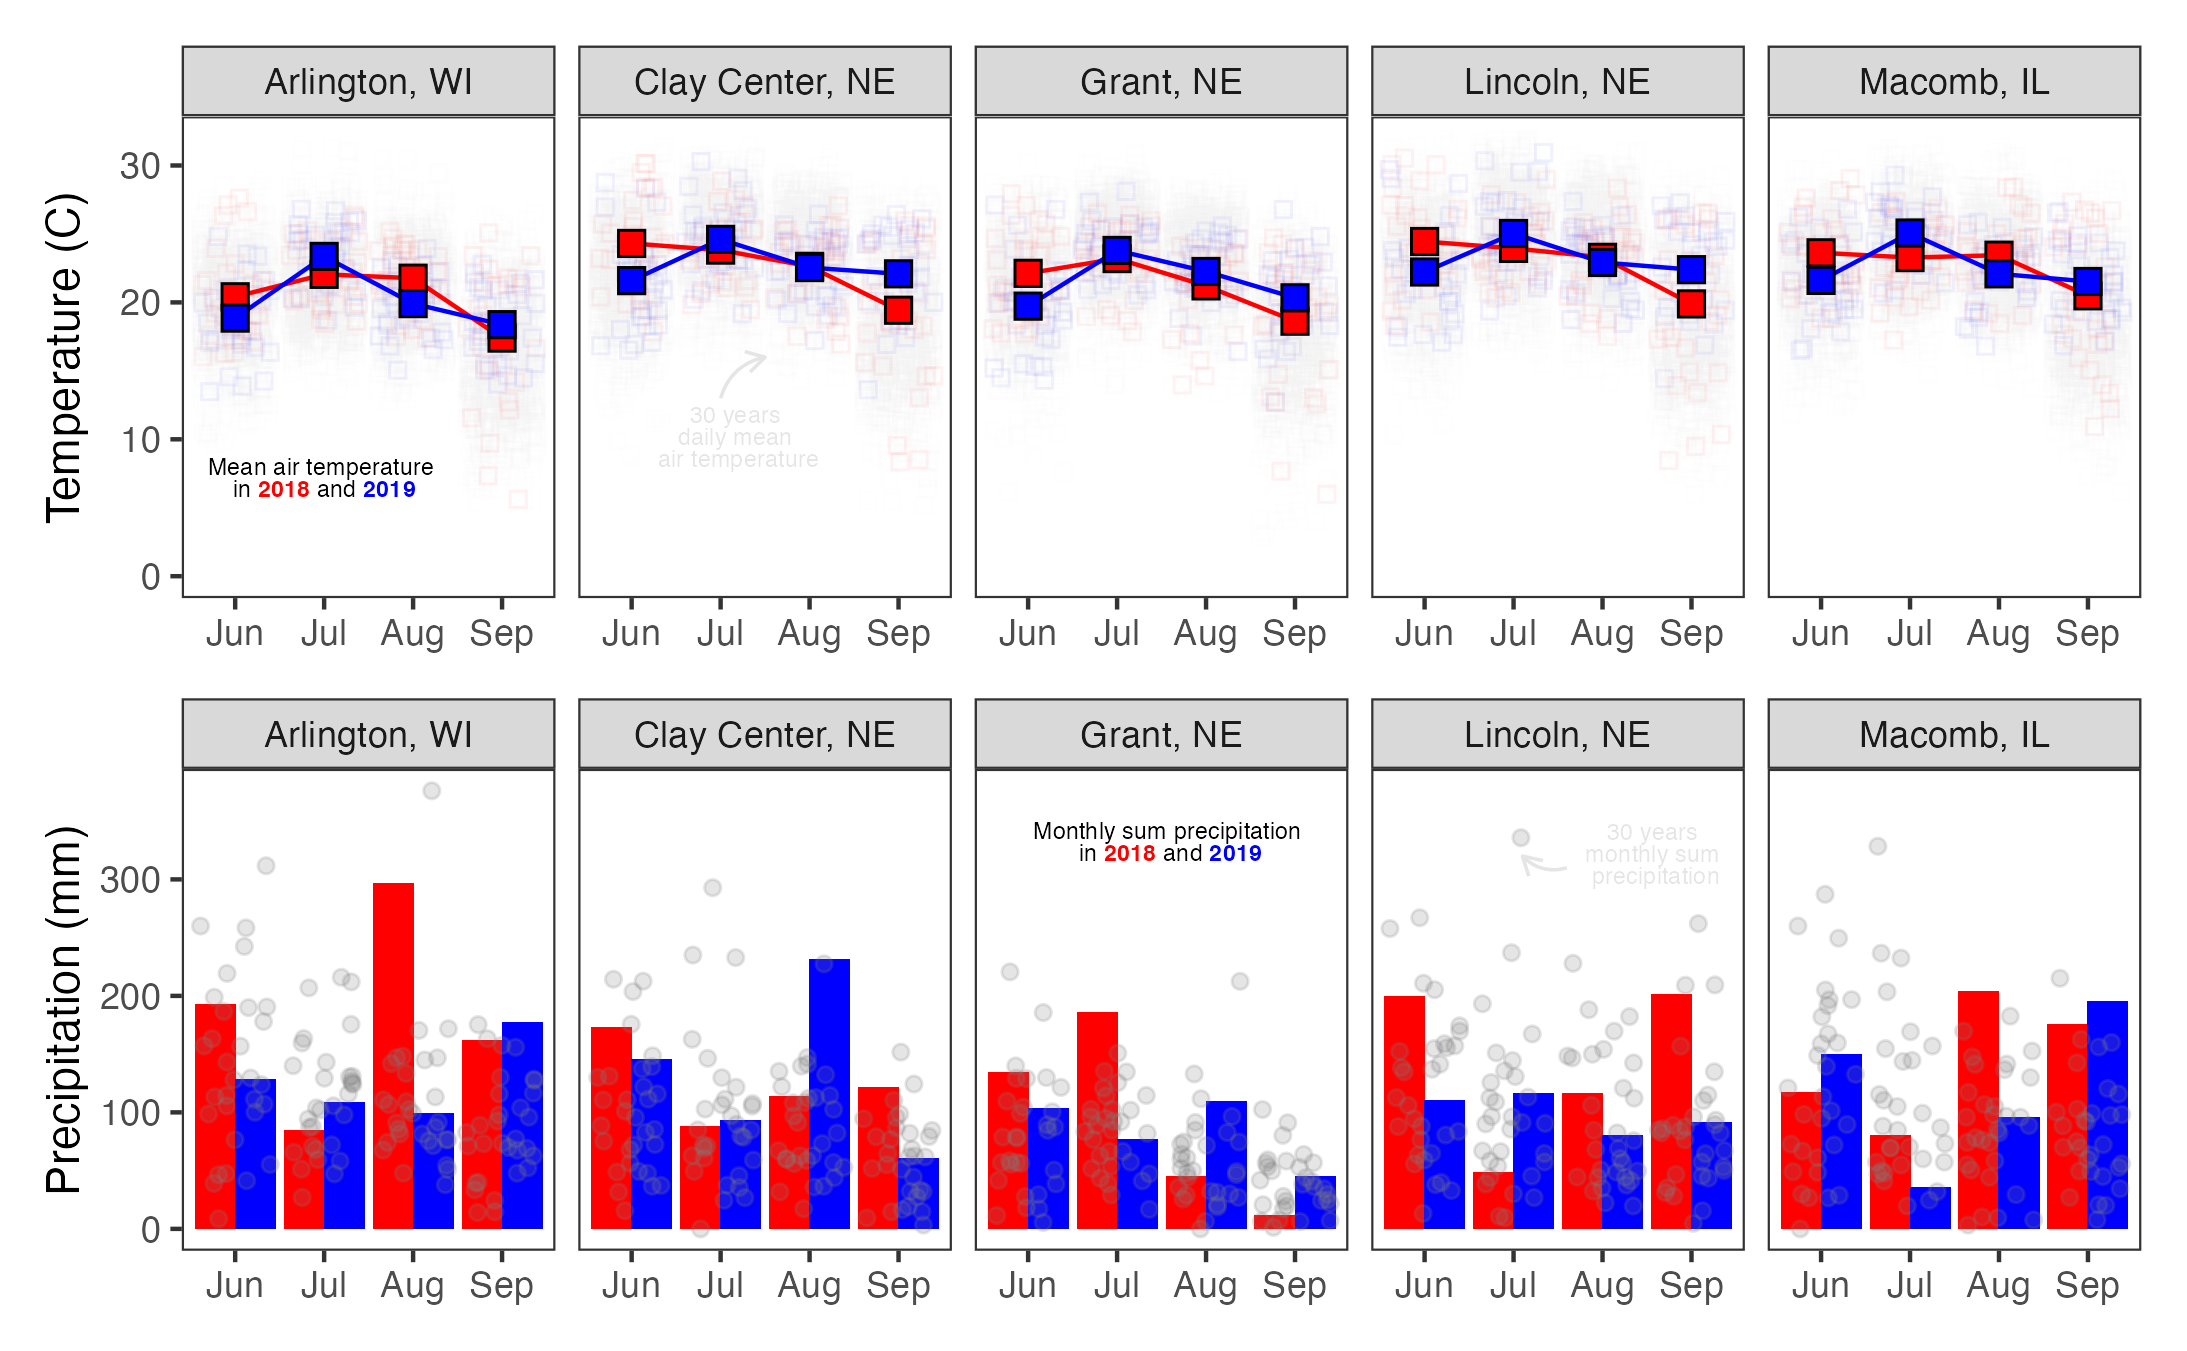
\includegraphics[width=160mm,height=100mm]{../data analysis/weather/Figure 1} 

}

\caption{Mean average temperature (C) and montly sum precipitation (mm) at Arlington, WI, Clay Center, NE, Grant, NE, Lincoln, NE and Macomb, IL}\label{fig:Figure-1}
\end{figure}

\begin{figure}

{\centering 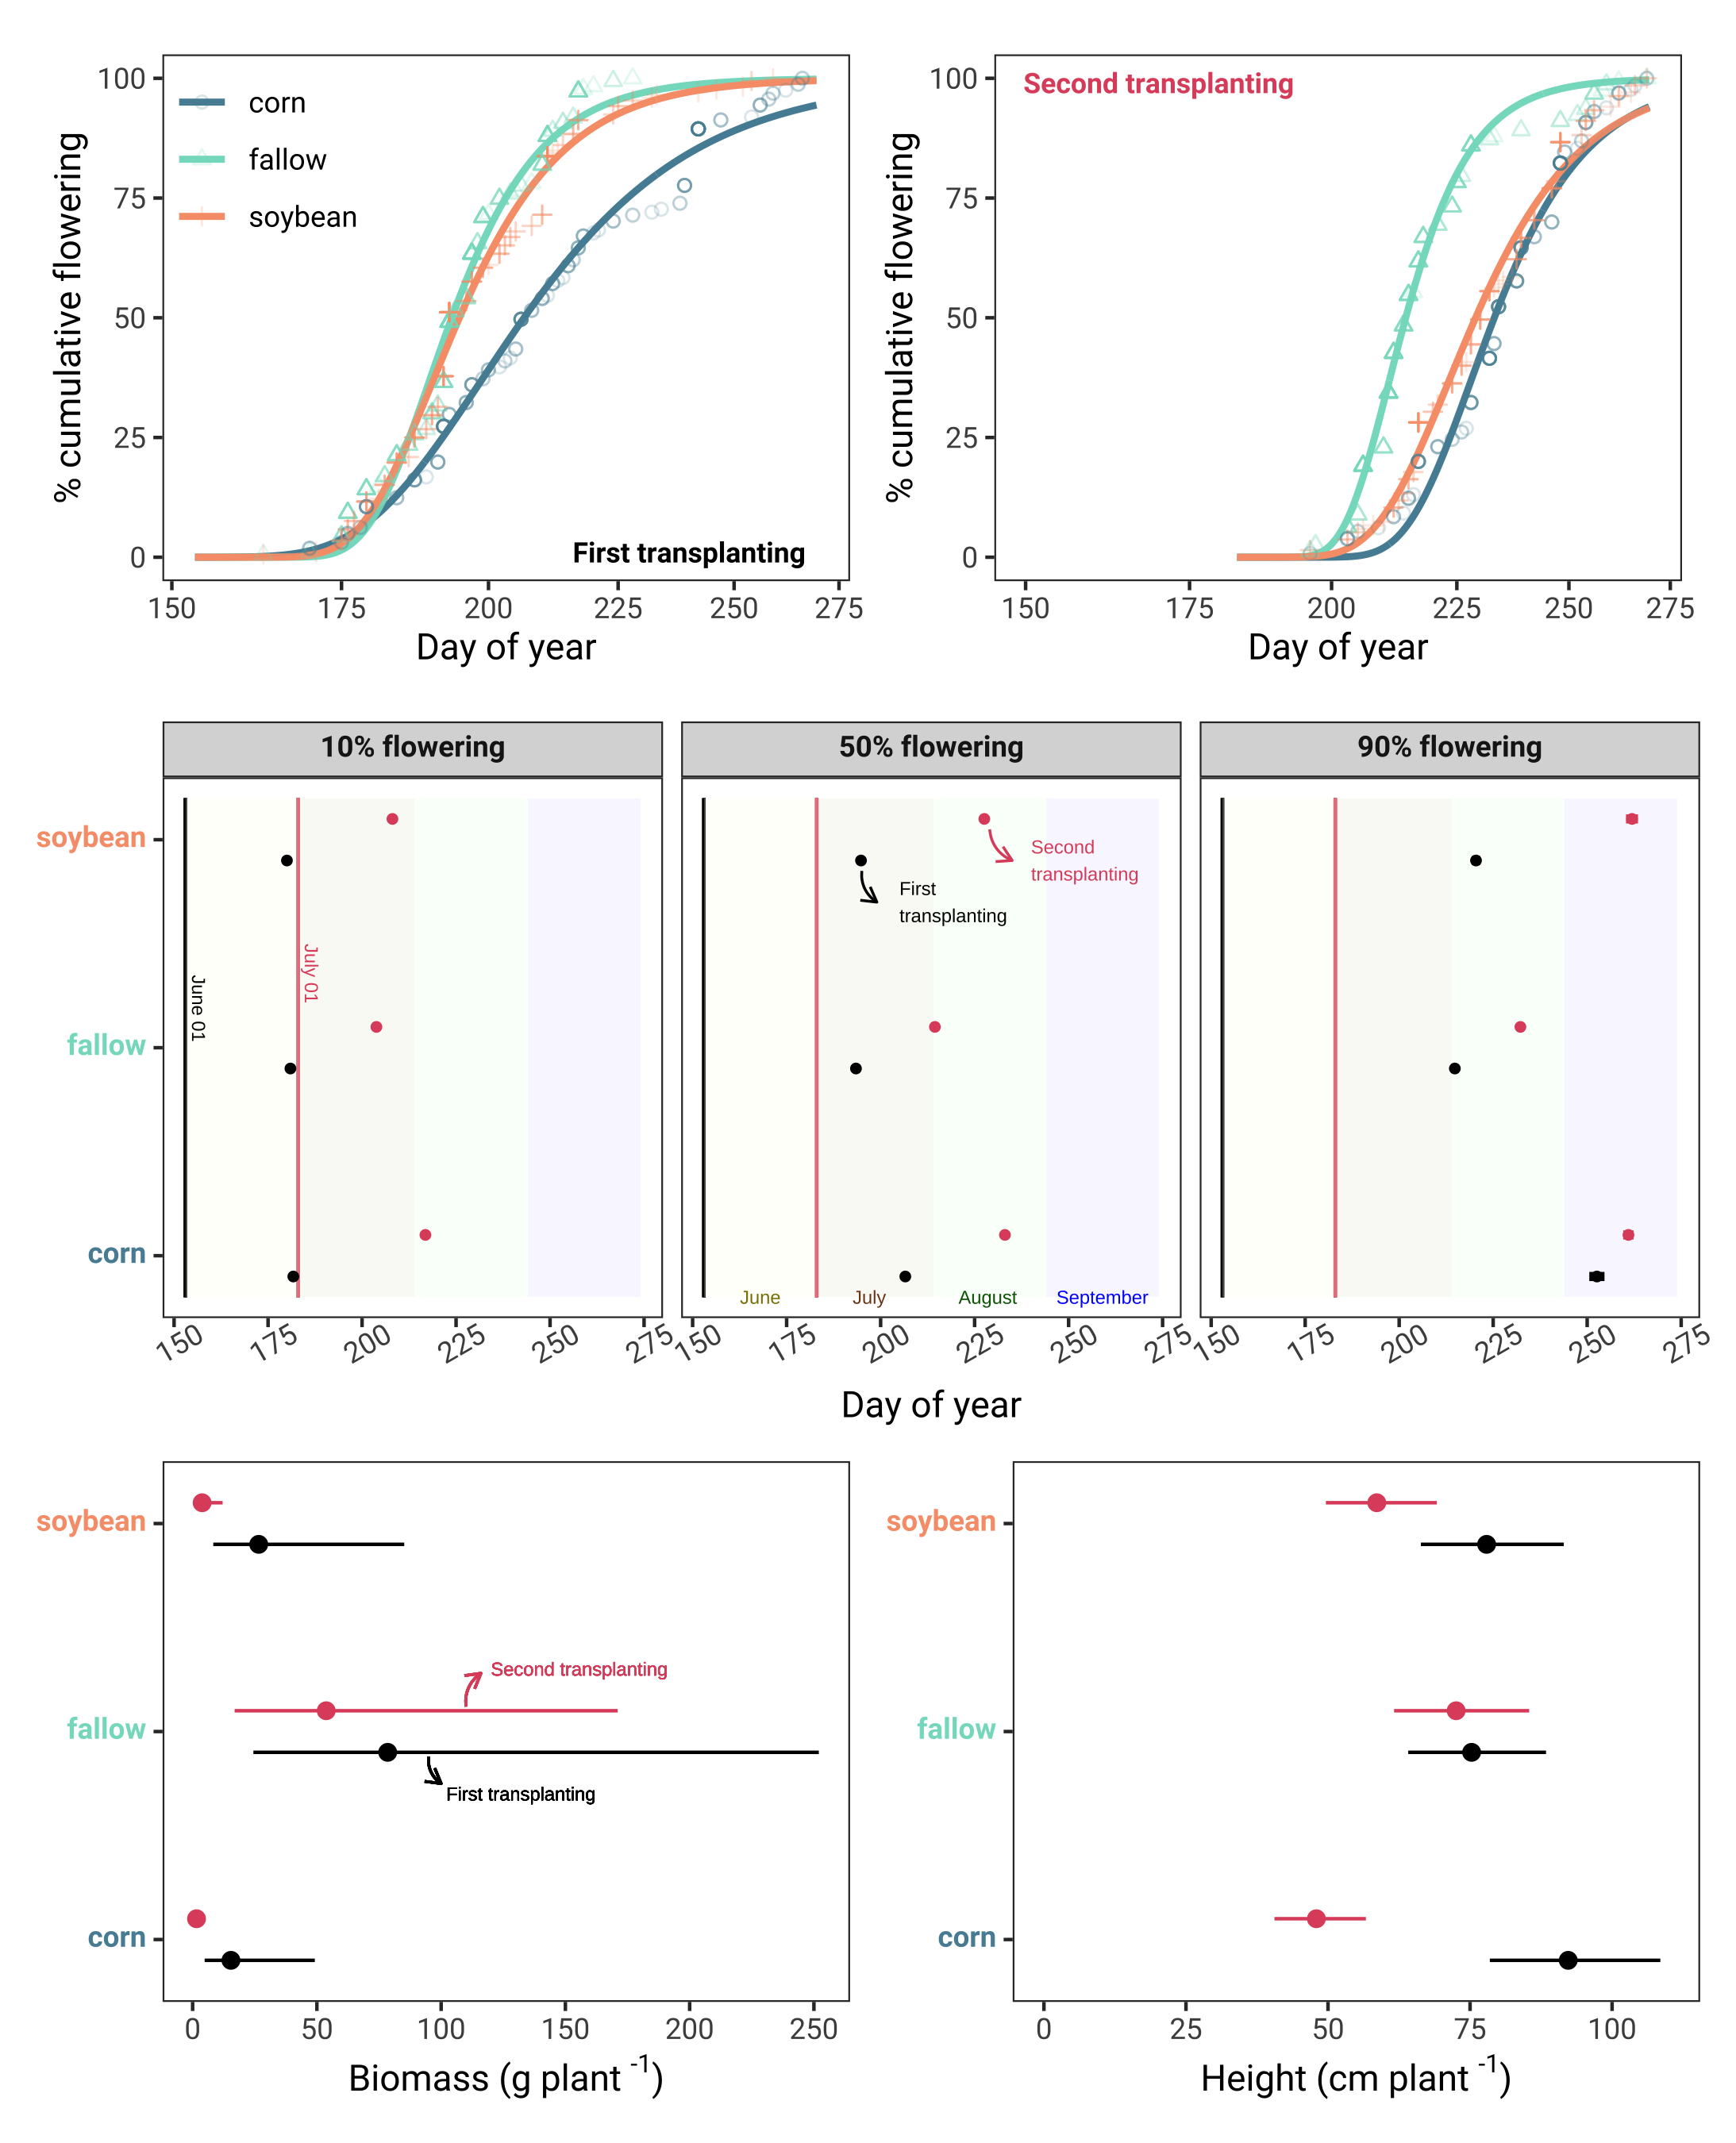
\includegraphics[width=150mm,height=260mm]{../data analysis/figures/combine 3} 

}

\caption{Figure caption}\label{fig:Figure-2}
\end{figure}

\hypertarget{refs}{}
\begin{CSLReferences}{1}{0}
\leavevmode\hypertarget{ref-oliveira2021a}{}%
Oliveira, M. C., Giacomini, D. A., Arsenijevic, N., Vieira, G., Tranel,
P. J., and Werle, R. (2021). Distribution and validation of genotypic
and phenotypic glyphosate and {PPO}-inhibitor resistance in {Palmer}
amaranth ({Amaranthus} palmeri) from southwestern {Nebraska}. \emph{Weed
Technology} 35, 65--76.
doi:\href{https://doi.org/10.1017/wet.2020.74}{10.1017/wet.2020.74}.

\leavevmode\hypertarget{ref-ritz2015}{}%
Ritz, C., Baty, F., Streibig, J. C., and Gerhard, D. (2015).
Dose-{Response Analysis Using R}. \emph{PLOS ONE} 10, e0146021.
doi:\href{https://doi.org/10.1371/journal.pone.0146021}{10.1371/journal.pone.0146021}.

\end{CSLReferences}

\end{document}
